\documentclass[11pt,a4paper]{article}
\usepackage{a4wide}
\usepackage{epsfig}
\usepackage{subfigure}

\usepackage[T1]{fontenc}
\usepackage[slovene]{babel}
\usepackage[utf8]{inputenc}
\usepackage{color,soul} %za označevanje besedila z rumenim markerjem
\usepackage{courier} %%za kodo v vrsticah (curier new)


\renewcommand{\topfraction}{1.}
\renewcommand{\bottomfraction}{1}
\renewcommand{\textfraction}{0.}
\renewcommand{\floatpagefraction}{1.}
\usepackage{color}

\usepackage{listings}
\definecolor{mygray}{rgb}{0.95,0.95,0.95}

\lstset{language=C} 
\lstset{frame=single}
\lstset{backgroundcolor=\color{mygray}}
\lstset{basicstyle=\footnotesize}
%%\lstset{keywordstyle=\color{red}}
\lstset{morekeywords={OUTPUT,digitalWrite, digitalRead,analogWrite,analogRead,pinMode, LOW, HIGH, INPUT, INPUT_PULLUP,digitalRead, delay, begin, setCursor, print, LiquidCrystal, noBlink}}
%\lstset{ title=\lstname}                   % show the filename of files included with \lstinputlisting; also try caption instead of title
\lstset{numbers=left}
\lstset{numbersep=5pt}                   % how far the line-numbers are from the code
\lstset{numberstyle=\tiny\color{blue}} % the style that is used for the line-numbers

   

\title{Programiranje z Arduinom in modulom RobDuino}
\author{Tomaž Kušar}
\date\today
\begin{document}
\maketitle
\thispagestyle{empty}
\newpage
\setcounter{page}{1}
\tableofcontents
\newpage

\section{Vmesnik Arduino in modul RobDuino}
Pri robotiki bomo uporabljali vmesnik Arduino UNO in modul RobDuino, ki nam omogoča prilop različnih senzorjev, krmiljenje motorjev, uporabo LCD-ja itd. Vmesnik ima vijačne sponke, kamor lahko povežemo žice senzorjev in aktuatorjev, ima pa tudi ženske in moške pinske priključke (iglične priključke), kamor lahko priključimo na primer servomotorje ali žice.

%\begin{figure}[h!] \centering
%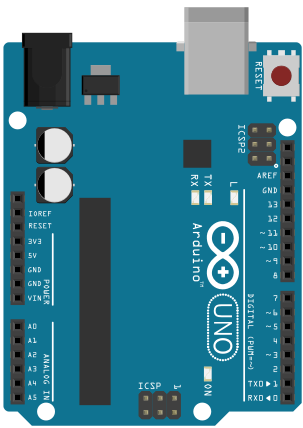
\epsfig{file=slike/ArduinoUNO.png,angle=0,clip=,width=5cm}
%\caption{Arduino UNO R3}\label{slika:arduinouno}
%\end{figure}

\begin{figure}[h] %h je zato, da so slike točno na tem mestu, da jih ne zmeče po svoje
\centering
\parbox{5cm}{
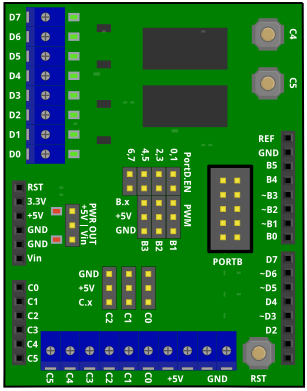
\epsfig{file=slike/robduino_board.png,angle=0,clip=,width=5cm}
\caption{Modul RobDuino.}\label{slika:robduino_board}
\label{slika:robduino_board}}%
\qquad
\begin{minipage}{5cm}
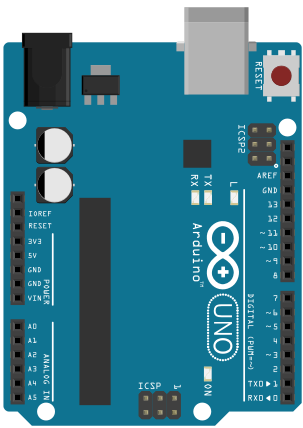
\epsfig{file=slike/ArduinoUNO.png,angle=0,clip=,width=5cm}
\caption{Arduino UNO R3}\label{slika:arduinouno}
\label{slika:arduinoUNO}%
\end{minipage}%
\end{figure}


Modul RobDuino nam omogoča uporabo skoraj vseh funkcij, ki jih omogoča Arduino UNO oziroma mikrokrmilnik ATmega328p. V začetku so prikazane osnovne funkcije, v nadaljevanju pa še naprednejše, ki so namenjene poznavalcem oziroma najbolj zagrizenim.  

S slike \ref{slika:robduino_board} je moč razbrati, da ima modul ob straneh drugačne oznake pinov, kot vmesnik Arduino UNO. V tej skripti se bomo sklicevali na oznake pinov kot jih ima vmesnik Arduino UNO, torej označene s številkami od 0 do 19. Pin 7 je na modulu označen z oznako D7, pin 8 pa je na modulu označen z oznako B0.   

Modul RobDuino nam omogoča uporabo skoraj vseh funkcij, ki jih omogoča Arduino UNO oziroma mikrokrmilnik ATmega328p. V začetku so prikazane osnovne funkcije, v nadaljevanju pa še naprednejše, ki so namenjene poznavalcem oziroma najbolj zagrizenim.  
Modul RobDuino nam omogoča uporabo skoraj vseh funkcij, ki jih omogoča Arduino UNO oziroma mikrokrmilnik ATmega328p. V začetku so prikazane osnovne funkcije, v nadaljevanju pa še naprednejše, ki so namenjene poznavalcem oziroma najbolj zagrizenim.  



\section{Digitalni izhod - vklop lučke}
Vmesnik Arduino oziroma modul RobDuino ima 19 uporabnih vhodno/izhodnih priključkov. Na modulu RobDuino so nekateri od njih podvojeni ali pa še celo potrojeni, ampak več o tem v nadaljevanju.

Digitalni izhod postavimo v logično 1 z ukazom \texttt{\textbf{digitalWrite(pin,stanje)}}, kjer pin pomeni oznaka priključka, stanje pa je lahko samo logična 1 ali logična 0. Če je izhod v logični 1, potem imamo na tem izhodnem priključku napetost +5V. Na priključkih od 0 do 7 so te napetosti v našem primeru lahko višje, odvisne od napajelne napetosti vmesnika Arduino, recimo +9V. Da nek priključek lahko uporabljamo kot izhod, ga moramo pred tem ustrezno konfigurirati, kar storimo z ukazom \texttt{\textbf{pinMode(pin,OUTPUT)}}.

Spodaj je primer programa s katerim postavimo pin 2 v logično 1 in nazaj v logično 0. 


\begin{lstlisting}
void setup() {
  // put your setup code here, to run once:
  pinMode(2, OUTPUT);
}
void loop() {
  digitalWrite(2, 1);
  delay(200);
  digitalWrite(2,0);
  delay(200);
}
\end{lstlisting}

Če program uspešno prenesemo v mikrokrmilnik, utripa ledica z oznako D2. 


\section{Digitalni vhod - branje tipke, stikala}
Za branje digitalnega vhoda uporabljamo ukaz \texttt{\textbf{digitalRead(pin)}}, kjer je pin oznaka priključka. Tako kot pri digitalnem izhodu, moramo tudi pri digitalnem vhodu najprej priključek definirati kot vhodni. Običajna konfiguracija je zapisana v 4. vrstici. Ker pa sta na modulu RobDuino dve tipki že nameščeni tako, da skleneta vhodni priključek 18 in 19 z GND, če jih sklenemo, smo vhodni priključek programsko povezali z uporom proti +5V. Tej vezavi rečemo Pull-up vezava. Arduino ima za to posebej namenjeno funkcijo in sicer \texttt{\textbf{pinMode(pin, INPUT\_PULLUP)}}.

\textit{OPOMBA: Vedno, ko uporabljamo tipki C4(pin18) in C5(pin19) uporabimo pull-up vezavo.}

\begin{lstlisting}
void setup() {
  pinMode(2, OUTPUT);
  pinMode(19, INPUT_PULLUP);
  //pinMode(19, INPUT);
  //digitalWrite(19, 1); //pull-up
}
void loop() {  
  if (digitalRead(19) == 0) {
    //vklopi LED
    digitalWrite(2, 1);
  } else {
    // izklopi LED
    digitalWrite(2, 0);
  } 
}
\end{lstlisting}
Če program uspešno prenesemov  mikrokrmilnik, sveti LED z oznako D2, ko sklenemo tipko C5.w


\section{Analogni vhod - branje senzorja}
Vmesnik Arduino ima na voljo 6 analognih vhodov na priključkih od 14 do 19. Na modulu RobDuino so označeni z C0, C1..., C5. Ti priključki se na modulu tudi podvojijo in jih najdemo na igličnih konektorjih, na vijačnih sponkah kot tudi na žensih igličnih konektorjih.
Na vmesniku ArduinoUNO so analogni vhodi poimeovani z oznakami od A0 do A5. Ko v programu zapišemo da uporabljamo pin A0, program ve, da gre za analogni vhod. Ker so priključki prvotno nastavljeni kot vhodi, nam ni potrebno posebej konfigurirati vhodov. Dovolj je, da poznamo ukaz \texttt{\textbf{analogRead(anPin)}}, kjer \textbf{anPin} označuje številko analognega vhoda. Spodaj je primer programa branja analognega vhoda A0. Vrednost analognega vhoda hranimo v spremenljivki tipa integer (prva vrstica programa).  


\begin{figure}[h!] \centering
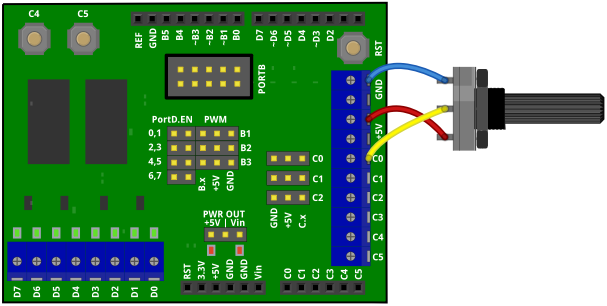
\epsfig{file=slike/potenciometer.png,angle=0,clip=,width=10cm}
\caption{Branje analognega vhoda - potenciometer}\label{slika:potenciometer}
\end{figure}


\begin{lstlisting}
int sensorValue = 0; //spremenljivka, kjer hranimo vrednost analognega vhoda

void setup() {
  // put your setup code here, to run once:
  pinMode(7, OUTPUT);
}
void loop() {  
  sensorValue = analogRead(A0);
  digitalWrite(7, 1);
  delay(sensorValue);
  digitalWrite(7,0);
  delay(sensorValue);  
}
\end{lstlisting}
Če smo program uspešno prenesli v mikrokrmilnik, potem je hitrost utripanja LED-ice z oznako D7 odvisna od vrednosti analognega vhoda. 

\section{Analogni izhod - krmiljenje moči}
Krmiljenje moči porabnika je malce zahtevnejše. Na tem mestu bomo samo povedali, kakšni so ukazi za nastavljanje analognega izhoda, podobnosti pa bomo pojasnili v nadaljevanju.
Ukaz s katerim nastavimo moč na izhodnem pinu je \texttt{\textbf{analogWrite(pin, power)}}, pri čemer je pin izhodni priključek, power pa je številka, s katero nastavljamo moč izhoda[0-255].
Z imenjenimi priključki lahko krmilimo manjše porabnike, recimo LED-ice. Če pa želimo moč nastavljati tudi na večjih porabniki, na primer motorjih, moramo v kombinaciji z PWM pini nastaviti tudi določene izhodne pine [0 do 5]. 

 

\begin{lstlisting}
/*
 Fade

 This example shows how to fade an LED on pin 9
 using the analogWrite() function.

 The analogWrite() function uses PWM, so if
 you want to change the pin you're using, be
 sure to use another PWM capable pin. On most
 Arduino, the PWM pins are identified with 
 a "~" sign, like ~3, ~5, ~6, ~9, ~10 and ~11.

 This example code is in the public domain.
 */

int led = 10;           // the PWM pin the LED is attached to
int m1a = 3;

int brightness = 0;    // how bright the LED is
int fadeAmount = 5;    // how many points to fade the LED by

// the setup routine runs once when you press reset:
void setup() {
  // declare pin 9 to be an output:
  pinMode(led, OUTPUT);
  pinMode(3, OUTPUT);
  pinMode(2, OUTPUT);
  int m1a = HIGH;
  digitalWrite(3, 1);
}

// the loop routine runs over and over again forever:
void loop() {
  // set the brightness of pin 9:
  analogWrite(led, brightness);

  // change the brightness for next time through the loop:
  brightness = brightness + fadeAmount;

  // reverse the direction of the fading at the ends of the fade:
  if (brightness <= 0 || brightness >= 255) {
    fadeAmount = -fadeAmount;
  }
  // wait for 30 milliseconds to see the dimming effect
  delay(30);
\end{lstlisting}






\section{LCD zaslon}
Na modul RobDuino lahko priključimo tudi LCD zaslon. Temu je namenjen 10 pinski konektor. V kolikor uporabljamo LCD zaslon, ne moremo uporabljati priključkov 8, 9, 10, 11, 12 in 13. Vse te priključje uporablja LCD zaslon. To pa pomeni, da ne moremo uporabljati tudi analognih izhodov na pinih 9, 10 in 11. 

\begin{figure} \centering
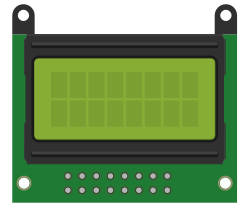
\epsfig{file=slike/lcd.png,angle=0,clip=,width=5cm}
\caption{LCD 8 x 2}\label{slika:lcd}
\end{figure}

\begin{lstlisting}
/*
 Vezava:
 * LCD RS pin to digital B3 ~  pin 11
 * LCD Enable pin to digital B2  ~ pin 10
 * LCD D4 pin to digital B5  ~ pin 13
 * LCD D5 pin to digital B1 ~ pin 9
 * LCD D6 pin to digital B4 ~ pin 12
 * LCD D7 pin to digital B0 ~ pin 8
 * LCD R/W pin to ground
 * 10K resistor:
   * ends to +5V and ground
   * wiper to LCD VO pin (pin 3)
 */

// include the library code:
#include <LiquidCrystal.h>
// inicializacija LCD-ja in dolocitev pinov za LCD
LiquidCrystal lcd(11, 10, 13, 9, 12, 8);

void setup() {
  lcd.begin(8, 2); // nastavitev LCD-ja (najprej stolpci, potem vrstice)
  lcd.print("Zdravo");
  lcd.setCursor(0, 1); // postavimo kurzor na prvo mesto v drugi vrstici
  lcd.print("svet!");
}
void loop() {
	...
}
\end{lstlisting}







\maketitle
\end{document}